\documentclass[pdflatex,sn-basic]{sn-jnl}
\usepackage{graphicx}
\usepackage{amsmath,amssymb}
\usepackage{booktabs}
\usepackage{multirow}
\usepackage{hyperref}
\usepackage{xcolor}
\usepackage{listings}
\usepackage{pgfplots}
\pgfplotsset{compat=1.17}

\begin{document}

\title[Replay-verified connectome computation in a consent-gated sensing commons]{Machine-checkable ecological evidence: replay-verified computation over biological connectomes in a consent-gated sensing commons}

\author*[1]{\fnm{Thomas} \sur{Price}}\email{hello@templeearth.cc}
\affil*[1]{\orgname{Temple Earth (Treetable LLC)}, \state{Colorado}, \country{USA} \\ ORCID: \href{https://orcid.org/0009-0009-7108-919X}{0009-0009-7108-919X}}

\abstract{Ecological monitoring and biodiversity-credit markets depend on
evidence that a sensor reading was produced where and how it is claimed.
Existing approaches -- trusted firmware, third-party auditors, and
zero-knowledge or trusted-execution proof systems -- either require
field hardware trust or carry heavy proof-generation cost. We present
an alternative: \emph{replay-verified computation}, in which a
deterministic simulator executed over a preserved biological wiring
diagram produces a witness signature that any independent
implementation can reproduce bit-for-bit, and \emph{WiredReplay-1}, a
conformance corpus of fifteen packed connectomes (cellular
electron-microscopy and mesoscale parcellation) with canonical inputs
and expected digests for validating third-party simulators. The
witnesses sit inside a consent-gated sensing commons that separates
evidence-gated lanes (sensing, fleet aggregation) from consent-gated
lanes (emission to and storage on living systems) and refuses the rest
as first-class protocol values. We demonstrate: (i) fifteen of
fifteen connectomes relay a shared feature-vector input with fifteen
topology-unique signatures, replayed identically by independent
Python and TypeScript implementations (930/930 parity checks);
(ii) at the largest cellular wiring, the packed simulator uses
$\sim$10$^3\times$ fewer estimated joules than an equivalent dense fp32
multiply on the same host, while a degree-matched shuffled control
shows the saving comes from sparse packed representation, not
biological topology -- a negative result we report deliberately;
(iii) the full protocol is exercised by 121 end-to-end checks and a
live public deployment (71/71 checks) exposing content-addressed,
receipt-gated verdicts. A small-wiring benchmark where our approach
\emph{loses} (Celegans, 302 neurons) is reported alongside the win.
The corpus, specification, harnesses, and claim-evidence table are
open (AGPL/CC-BY), pre-registered in the accompanying methods
repository, and intended as a citable standard for deterministic
biologically-derived computation.}

\keywords{connectome, spiking neural simulation, determinism, replay
verification, provenance, ecological monitoring, MRV, consent,
open science}

\maketitle

\section{Introduction}\label{sec:intro}
Ecological sensing is scaling faster than the evidence discipline that
would make its outputs trustworthy. Autonomous acoustic recorders,
eDNA samplers, and community-sensor networks now generate continuous
streams of claimed observations about living systems
\cite{hill2018,sueur2015,kahl2021}; biodiversity-credit and
conservation-finance markets are beginning to price claims derived
from those streams \cite{ford2024}. The evidentiary question ---
\emph{was this reading produced as claimed, by what, and under whose
authority?} --- is typically answered by trusting firmware and
auditors, or deferred to provenance standards that describe data
lineage without constraining it \cite{provo2013,wieczorek2012}.

We describe a sensing commons, \emph{Temple Earth}, in which the
evidence problem is treated as a verifiable-computation problem with
an unusual verifier: preserved biological wiring diagrams
(connectomes) replayed by deterministic simulation. The system is
built around three separable contributions.

First, a \textbf{protocol} in which every capability is routed through
one of two explicit gates. \emph{Evidence-gated lanes} (sensing,
fleet-wide aggregation) admit only inputs that carry a verifiable
provenance claim. \emph{Consent-gated lanes} (emission toward a living
system, storage on a guardian-controlled node) admit only operations
whose consent tuple --- guardian, operator, action class, policy
hash --- verifies at admission time. Lanes that satisfy neither
(including any computation claimed to run \emph{inside} a living
organism, and any relay that would write back into a sensed
environment) are \emph{refused as a first-class protocol value}: a
signed refusal is itself a receipt, auditable and quotable. Emission,
where permitted, is further constrained to minimal energy and
duty-cycled bursts under joint guardian and operator consent ---
``the emission stack is consent-gated, minimal, and duty-cycled; the
default posture is listen-only.''

Second, \textbf{witnesses}: a deterministic leaky
integrate-and-fire (LIF) simulator that runs the same packed graph
step-for-step on a commodity host or in a cloud worker, producing a
BLAKE2s digest of the full spike raster --- the \emph{witness
signature} of that wiring diagram under that input. Because the
simulation is deterministic by construction (fixed-point arithmetic,
no floating-point scheduling, no RNG state), any conformant
implementation reproduces the signature exactly; agreement between
independent implementations is a cryptographic-strength coincidence,
not a configuration detail. A quorum of witnesses --- distinct
connectomes agreeing on a verdict under quorum rules --- folds into a
single content-addressed evidence record (a \emph{receipt}, addressed
by self-authenticating identifier, SAID).

Third, \textbf{WiredReplay-1}: the corpus that makes the witness layer
a shared standard rather than a proprietary implementation detail ---
fifteen packed wiring diagrams, canonical test vectors with expected
digests, and the normative format and encoder specification.

\subsection{Claims and evidence discipline}
Every quantitative statement in this paper is labelled by the
evidence tier used throughout the project: \emph{proven by
science} (published external literature), \emph{built --- heading
outdoors} (implemented and tested, not field-deployed),
\emph{live now} (running in the deployed system), \emph{measured},
\emph{estimated}, \emph{cited}, \emph{projected}, or
\emph{refused}. The full claim table is Appendix~\ref{app:claims} and
the authoritative version is \texttt{docs/SCIENCE.md} in the
repository. Where our own method performs poorly --- and one such
case is deliberately included --- we report it.

\subsection{Contributions}
\begin{itemize}
\item A protocol architecture separating evidence-gated from
      consent-gated lanes, with signed refusal as a receipt
      (Section~\ref{sec:arch}, Appendix~\ref{app:spec}).
\item Deterministic replay-verified computation over fifteen
      preserved biological connectomes, with independent
      implementations agreeing on every digest (Sections
      \ref{sec:methods}, \ref{sec:results}).
\item WiredReplay-1, an open conformance corpus: packed graphs,
      checksums, 45 canonical vectors, expected digests, and the
      encoder specification (Section~\ref{sec:corpus}).
\item An honest efficiency analysis with a degree-matched shuffled
      control showing the measured gain is from sparse packed
      representation, not biological topology
      (Section~\ref{sec:efficiency}).
\item A threat model and claim-evidence table that bind every
      statement to its tier (Appendices \ref{app:threat},
      \ref{app:claims}).
\end{itemize}

\section{Related work}\label{sec:related}
\textbf{Connectomes at both resolutions.} Cellular-scale wiring is now
available for \emph{C.\ elegans} (both sexes)
\cite{white1986,cook2019}, tadpole \emph{Ciona} \cite{ryan2016},
\emph{Drosophila} larva \cite{ohyama2015,gerhard2017} and adult
(hemibrain \cite{scheffer2020}, full FAFB/FlyWire
\cite{zheng2018,dorkenwald2024}), \emph{Platynereis}
\cite{veraszto2020}, and mouse retina \cite{helmstaedter2013};
medulla-column data derive from Takemura et al.\
\cite{takemura2015}. Mesoscale matrices exist for mouse
\cite{oh2014}, rat \cite{bota2015}, macaque
\cite{markov2014,modha2010}, human \cite{hagmann2008}, and cat
\cite{scannell1993}. Prior work uses these graphs for circuit
neuroscience; we use them as deterministic witnesses --- a
\emph{representation} claim about reproducible computation, not a
claim about cognition or ecology.

\textbf{Simulation and reservoir computing.} The LIF step is a
standard discrete membrane equation \cite{hh1952,brette2007,izhikevich2003}.
Using recurrent wiring as an untrained readout substrate is reservoir
computing \cite{jaeger2001,maass2002,lukosevicius2009}; OpenWorm
demonstrates whole-animal simulation as an open-science artifact
\cite{szigeti2014}. Our contribution is not a simulator but a
\emph{verification discipline} around one: determinism requirements,
a conformance corpus, and digest-level replay.

\textbf{Neuromorphic baselines.} TrueNorth \cite{merolla2014}, Loihi
\cite{davies2018}, and SpiNNaker \cite{furber2014} run spiking
networks at low power on dedicated silicon. We deliberately compare
against same-host CPU baselines instead: the relevant question for an
edge sensing commons is whether \emph{this} representation is cheap
on the hardware already deployed.

\textbf{Verifiable computation.} Cryptographic verification spans
interactive proofs, succinct arguments \cite{groth2016}, and
trusted execution \cite{costan2016}; Walfish and Blumberg's survey
framed the trade-off: verify without re-executing, at a price in
proof cost or hardware trust \cite{walfish2015}. Certificate
Transparency showed the value of append-only, publicly replayable
logs for a different domain \cite{laurie2014}, and supply-chain
frameworks (in-toto \cite{intoto2019}) popularized
receipted-build attestations. Our point of comparison:
where proof systems sell \emph{verification without re-execution},
we sell the opposite --- \emph{re-execution as the receipt} ---
which is viable precisely because the deterministic witness is
small (the largest blob is 1.08 MB) and the replay is cheap.

\textbf{Provenance and data standards.} PROV-O \cite{provo2013} and
Darwin Core \cite{wieczorek2012} describe lineage and occurrence
records; FAIR \cite{wilkinson2016} governs discoverability; CARE
\cite{carroll2020} governs consent for data about communities. Our
consent gate operationalizes a CARE-style principle --- collective
benefit, authority to control --- as an executable admission rule
rather than a documentation requirement.

\textbf{Ecological sensing and MRV.} Open acoustic hardware
\cite{hill2018,pearce2012}, bird-sound classifiers \cite{kahl2021},
and ecoacoustic indices \cite{sueur2015} supply the sensing frontier;
MRV criteria (e.g.\ SAGED \cite{ford2024}) define what counts as
credible evidence. The living-systems lane claims motivating our
gate design --- airborne plant stress sounds \cite{khait2023},
biofilm ion-channel waves \cite{prindle2015}, biofilm-to-biofilm
coupling \cite{liu2017}, electrical cell attraction
\cite{humphries2017}, and contactless conductivity sensing
\cite{kuban2009} --- are catalogued per-claim in
Appendix~\ref{app:claims}. This paper claims none of them as inputs;
they motivate why the consent lane exists.

\textbf{Positioning.} Table~\ref{tab:compare} summarizes the
verification landscape.

\begin{table}[t]
\centering\small
\caption{Verification approaches for remote environmental claims.}
\label{tab:compare}
\begin{tabular}{@{}llll@{}}
\toprule
 & proof cost & trust root & field cost \\
\midrule
Trusted firmware/auditor & none & vendor + auditor & low \\
ZK / SNARK \cite{groth2016} & high (proving) & math & high \\
TEE \cite{costan2016} & low & chip vendor & moderate \\
\textbf{This work} & \textbf{re-execution}
 & \textbf{determinism} & \textbf{low} \\
 & & \textbf{+ open corpus} & \\
\bottomrule
\end{tabular}
\end{table}

\section{The protocol}\label{sec:arch}
\subsection{Lanes and gates}
Every operation in the commons is assigned a lane, and every lane
satisfies exactly one gate (formal specification in
Appendix~\ref{app:spec}):
\emph{sense} (a sensor reports an observation),
\emph{fleet} (siblings corroborate an observation), and the refused
\emph{compute} lane (claiming an organism computed) are
\emph{evidence-gated}: admission requires a verifiable evidence claim.
\emph{emit} (drive a transducer toward a living system) and
\emph{store} (write on a guardian-controlled node) are
\emph{consent-gated}: admission requires a consent tuple
$\langle$guardian, operator, action-class, policy-hash$\rangle$ that
verifies at admission. \emph{hop} (relaying through living tissue)
and any claim of in-organism computation or storage are refused
unconditionally, as is promotion of a federated receipt to local
quorum status. A refusal is a signed, content-addressed protocol
value --- it is \emph{data}, not silence.

\subsection{Witnesses, quorum, receipts}
A sensing input is rasterized into a feature vector
$\langle$confidence, event-rate, env-anomaly, fleet-agreement$\rangle$
(Section~\ref{sec:methods}) and replayed through each admitted
connectome witness. Each witness emits a verdict:
$(\text{action} \in \{-1,0,+1\},\ \text{confidence},
\ \text{spike-count},\ \text{digest})$. A quorum is $\ge 3$
distinct connectomes agreeing on action; quorum output folds into a
receipt addressed by BLAKE2s SAID --- self-authenticating: the
address is the content's hash, so any holder can verify integrity
without trusting the store. Receipts are the unit mutual credit
settles against: a sensed detection contributes to credit only
through a witnessed, receipted record, never an unwitnessed claim.

\subsection{Custody}
Guardians hold custody of deployed nodes; operators hold keys for
service accounts; subjects (living systems) earn credit. Consent is
consent of the \emph{custodian}, never attributed to the organism ---
the model is explicit about this boundary and the paper makes no
claim of organism agency.

\section{Connectome witnesses: methods}\label{sec:methods}
\subsection{Corpus}\label{sec:corpus}
WiredReplay-1 contains fifteen wiring diagrams spanning two
resolution classes, deliberately not blurred: cellular EM
reconstructions (302--40{,}000 neurons) and mesoscale parcellation
graphs (49--242 neurons). Table~\ref{tab:datasets} lists the corpus;
Appendix~\ref{app:spec} gives the normative packed format.
Blob sizes are 4.9 KB--1.08 MB (packed int4-CSR): the entire cellular
medulla wiring fits in a megabyte.

\begin{table}[t]
\centering\small
\caption{WiredReplay-1 corpus. Resolution is stated per dataset;
``mesoscale'' graphs are interareal parcellations, not cellular
EM. Janelia-derived blobs (hemibrain, medulla, larva) are CC-BY
redistributable; cellular-scale rows are ``published-plausible''
(matches to published connectomes by size and count); the five
mesoscale rows drosophila, human, mouse, rat and macaque carry
\emph{provenance-pending} status --- their upstream
sources could not be re-identified from the packed artifacts, and the
corpus flags them accordingly rather than asserting an unverified
source. Determinism results do not depend on provenance; dataset
licensing status is tracked in \texttt{paper/datasets.md}.}
\label{tab:datasets}
\begin{tabular}{@{}lrrl@{}}
\toprule
connectome & neurons & synapses & resolution \\
\midrule
medulla          & 40{,}000 & 399{,}950 & cellular EM \\
hemibrain        & 21{,}636 & 216{,}310 & cellular EM \\
platynereis      & 5{,}000  & 49{,}991  & cellular EM \\
larva            & 3{,}016  & 30{,}149  & cellular EM \\
mouse\_retina    & 1{,}124  & 90{,}009  & cellular EM \\
celegans\_male   & 575      & 5{,}305   & cellular EM \\
celegans\_herm   & 453      & 4{,}878   & cellular EM \\
celegans         & 302      & 3{,}009   & cellular EM \\
human            & 234      & 7{,}076   & mesoscale \\
macaque\_modha   & 242      & 4{,}090   & mesoscale \\
ciona            & 205      & 2{,}902   & cellular EM \\
mouse            & 112      & 6{,}542   & mesoscale \\
macaque          & 93       & 1{,}692   & mesoscale \\
rat              & 73       & 1{,}923   & mesoscale \\
drosophila       & 49       & 1{,}950   & mesoscale \\
\bottomrule
\end{tabular}
\end{table}

\subsection{Packed representation}
Graphs are packed as int4 CSR (indptr deltas, u16 indices, 4-bit
two's-complement weights, two per byte) in $\le$24{,}575-byte chunks
with a JSON sidecar --- a derivative of the MIT-licensed FlyBrain
pack format. Packing is the efficiency instrument: weights are
quantized to nibbles, addresses compressed to per-neuron deltas.

\subsection{Determinism contract}
A conformant simulator must satisfy, end-to-end: integer arithmetic
throughout (Q24 fixed-point, floor division, right-shift rescale ---
no floating point anywhere \cite{goldberg1991}); no RNG --- per-neuron
input variation derives deterministically via BLAKE2s from the neuron
index (encoder \texttt{lif-sensing-v1}, Appendix~\ref{app:spec});
a fixed step count per blob; and digests defined over the exact byte
serialization. Determinism is what makes \emph{replay} the receipt:
equal digests from independent implementations is an
astronomically-unlikely coincidence, not agreement by tolerance.

\subsection{Replay protocol}
Given a verdict $\langle$connectome, input-SAID, features, steps,
action, confidence, spike-count, digest$\rangle$, a verifier
re-rasterizes the features, re-simulates, and compares digests
byte-for-byte. The deployed worker exposes this as a public
\texttt{/verify} endpoint; the corpus vectors replay the same way
offline.

\section{Results}\label{sec:results}
\subsection{E5: relay with topology-unique signatures}\label{sec:e5}
The pre-registered E5 criterion (an input relays through all
connectomes, each producing a distinct signature) \textbf{passed}:
15/15 relays, 15 distinct BLAKE2s signatures, replayed identically by
the Python reference runner and the TypeScript worker
(cross-implementation). The signatures are fingerprint-grade ---
two different wirings of the same input produce different digests ---
which is what lets a witnessed receipt distinguish \emph{which}
wiring diagram witnessed a claim.

\subsection{Cross-implementation parity}
The independent implementations agree on 930/930 parity checks
(feature grids over all 15 connectomes): identical actions,
confidences, and digests. Divergence observed in development ---
a documented keccak$\to$blake2s variation-source change between the
runner and its on-chain ancestor --- is a named encoder version
(\texttt{lif-sensing-v1}), demonstrating the corpus's intended use:
differences are caught at digest granularity and versioned.

\subsection{Protocol and deployment}
The five e2e suites (connectome witness, federation, refused lanes,
sensing cell, write lanes) total 121 checks, all passing under GNU
Guile 3.0. The live worker passed 71/71 checks against the production
deployment at templeearth.cc, including a live quorum$\to$verdict
round-trip and public \texttt{/verify} replay of a production
receipt (``live now'' tier; logs in \texttt{paper/artifacts/}).

\subsection{Efficiency, honestly}\label{sec:efficiency}
Figure~\ref{fig:bench} and Table~\ref{tab:bench} report the two
benchmark legs on the same host (fresh runs in
\texttt{paper/artifacts/}; earlier measured-tier runs appear in
\texttt{docs/EFFICIENCY.md}). Fresh-run joules use a
CPU-time$\times$15\,W proxy and are labelled \emph{estimated}.

\textbf{Large wiring (medulla, 40k neurons).} The connectome leg:
882{,}532 ops over 1{,}079{,}875 packed bytes, 2.05 ms,
$3.07\times10^{-2}$ J (est.). Against same-host baselines: dense fp32
$1.6\times10^9$ ops / 6.4 GB / 115.8 ms / 38.1 J (est.); sparse CSR
399{,}950 ops / 2.4 MB / 1.34 ms / 0.27 J (est.). The connectome is
$\sim$56$\times$ faster and $\sim$1{,}200$\times$ cheaper than dense;
it sits between dense and sparse exactly where its op count predicts.

\textbf{The control is the finding.} A degree-matched shuffled
medulla (same neurons, same degree sequence, randomized targets)
produces statistically identical timing and energy (2.06 ms,
$3.08\times10^{-2}$ J) --- \emph{the saving is the sparse packed
representation, not the biological topology}. We report this
deliberately: what the biological wiring contributes is the
\emph{signature} (a unique, replayable fingerprint of a real evolved
wiring), not the speed.

\textbf{Small wiring (celegans, 302 neurons).} The honest loss: our
leg is \emph{slower} than both baselines (0.120 ms vs 0.007 dense /
0.008 sparse) --- Python+NumPy overhead dominates below a scale
threshold. There is a crossover (roughly, the regime where
$O(\text{steps}\times\text{synapses})$ sparse work beats the
$O(n^2)$ dense multiply and where interpreter overhead is
amortized); medulla is past it, celegans is not. Both legs, including
the loss, ship in the corpus vectors.

\begin{figure}[t]
\centering
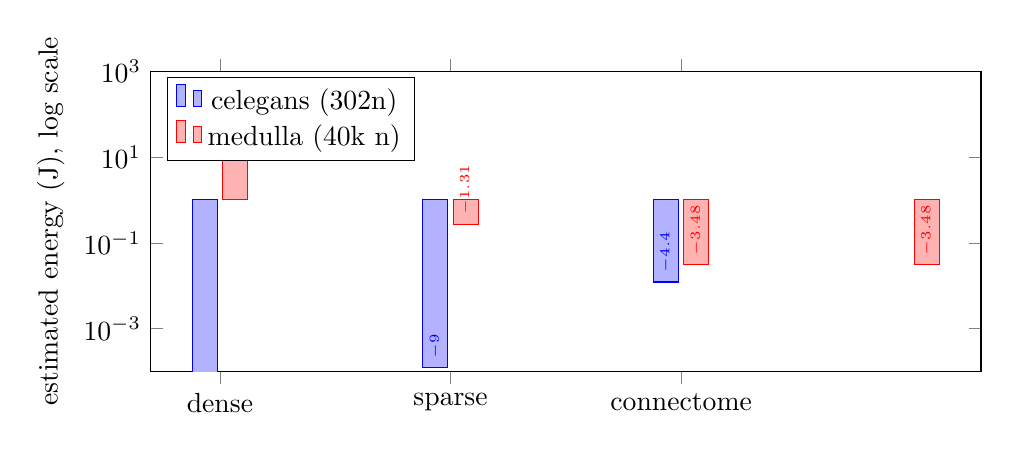
\begin{tikzpicture}
\begin{axis}[
    ybar, bar width=9pt, width=\linewidth, height=5.4cm,
    symbolic x coords={dense,sparse,connectome,shuffled},
    xtick=data, ylabel={estimated energy (J), log scale},
    ymode=log, ymin=1e-4, ymax=1e3,
    legend style={at={(0.02,0.98)},anchor=north west},
    nodes near coords, every node near coord/.append style={font=\tiny,rotate=90,anchor=west},
]
\addplot coordinates {(dense,9.77e-5) (sparse,1.23e-4) (connectome,1.23e-2)};
\addlegendentry{celegans (302n)}
\addplot coordinates {(dense,38.1) (sparse,0.271) (connectome,0.0307) (shuffled,0.0308)};
\addlegendentry{medulla (40k n)}
\end{axis}
\end{tikzpicture}
\caption{Estimated energy per simulation run (CPU-time$\times$15\,W
proxy). At cellular scale the connectome leg is $\sim$3 orders of
magnitude cheaper than dense; at 302 neurons it loses to both
baselines --- reported as the scale-limit honesty case. The
degree-matched shuffled control overlaps the real wiring, showing the
saving is representation, not topology.}\label{fig:bench}
\end{figure}

\begin{table}[t]
\centering\small
\caption{Benchmark legs, fresh runs (tier: \emph{estimated}). Ops
counts are semantic synaptic updates vs.\ MACs; ``shuffled'' is the
degree-matched control. Estimated joules are
CPU-time$\times$15\,W --- the multithreaded BLAS baselines burn
substantially more CPU-time than wall-time (dense: 2{,}540 ms CPU /
115.8 ms wall; sparse: 18.0 ms CPU / 1.34 ms wall), while the
connectome leg is single-threaded (2.04 ms CPU / 2.05 ms wall).
Wall-time figures therefore tell a different story than the energy
column --- sparse CSR is marginally faster on the wall clock but
$\sim$9$\times$ more expensive in CPU-joules.}\label{tab:bench}
\begin{tabular}{@{}llrrr@{}}
\toprule
wiring & leg & ops & bytes & est.\ J \\
\midrule
\multirow{4}{*}{medulla}
 & dense fp32  & $1.6\!\times\!10^9$ & $6.4\!\times\!10^9$ & 38.1 \\
 & sparse CSR  & 399{,}950 & 2{,}399{,}700 & 0.271 \\
 & connectome  & 882{,}532 & 1{,}079{,}875 & 0.0307 \\
 & shuffled    & 882{,}532 & 1{,}079{,}875 & 0.0308 \\
\midrule
\multirow{3}{*}{celegans}
 & dense fp32  & 91{,}204 & 364{,}816 & $9.8\!\times\!10^{-5}$ \\
 & sparse CSR  & 3{,}009  & 18{,}054  & $1.2\!\times\!10^{-4}$ \\
 & connectome  & 35{,}346 & 7{,}825   & $1.2\!\times\!10^{-2}$ \\
\bottomrule
\end{tabular}
\end{table}

\section{Discussion}\label{sec:disc}
\subsection{What the witnesses are --- and are not}
A witness signature certifies that \emph{this wiring diagram, under
this input, produced this raster}. Quorumed, it supports a claim that
a sensed observation was processed through a documented, replayable
pipeline. It does not certify that an organism computed, relayed, or
consented --- the connectome is a preserved wiring \emph{used as}
computation; the organism is not claimed as the computer. This
distinction is enforced in the protocol's lane table (living-system
compute is refused) and in the claim labels.

\subsection{The living cloud, honestly bounded}
The architecture is designed so that a future E0+ deployment ---
sensors reading living systems, consent-gated emission, receipts
crediting subjects --- plugs into the receipt machinery demonstrated
here without protocol changes. What this paper demonstrates is the
verifiable spine: provenance that degrades into refusal rather than
into trust, and a witness layer cheap enough to replay anywhere.
Field validation is explicitly out of scope (Section~\ref{sec:lim}).

\subsection{Threat model}
Appendix~\ref{app:threat} details adversary classes; the load-bearing
property is that \emph{forgery requires either breaking BLAKE2s or
defeating determinism}, while the honest-participant failure modes
(mis-rasterized input, wrong blob version) are detectable at digest
granularity. The residual trust point is the sensor itself ---
identical in kind to every remote-sensing system, and why the
evidence gates exist upstream of the witnesses.

\subsection{Limitations}\label{sec:lim}
(i) No field deployment: E0--E6 are pre-registered; none of the
``living'' lanes has produced a witnessed real-world receipt.
(ii) Estimated joules: fresh benchmark runs use a power proxy; the
measured-tier numbers in \texttt{docs/EFFICIENCY.md} come from
RAPL-unlocked runs and are labelled accordingly.
(iii) The witness layer validates \emph{computation}, not
\emph{biology}: connectome verdicts carry no claim about cognition,
ecology, or the health of the source organism. (iv) Sole-author
project; the corpus is young. (v) Mesoscale and cellular graphs are
mixed in one corpus deliberately --- resolution is declared per row,
and any use must respect it.

\section{Availability}
Code (AGPL-3.0): \url{https://github.com/TerexitariusStomp/living-resources}
--- \texttt{tools/connectome/}, \texttt{workers/compute-api/},
\texttt{tests/e2e/}. Corpus + vectors + spec: \texttt{paper/corpus/},
archived at \url{https://doi.org/10.5281/zenodo.23681503} (release
\texttt{paper-v1}).
Reproduction commands: \texttt{paper/REPRODUCE.md}. Deployed API:
\url{https://templeearth.cc} (\texttt{/verify} is a live replay
endpoint). Claim ledger: \texttt{docs/SCIENCE.md};
pre-registered experiments: \texttt{docs/EXPERIMENTS.md}.

\section*{Acknowledgements}
The author used AI assistance (Devin, Cognition AI) for code
execution, artifact generation, and drafting support during
preparation of this manuscript and its accompanying software.
All scientific claims, experimental design, framing, and
conclusions are the author's own.

\section*{Ethics and consent}
No living system was instrumented, stimulated, or emitted at for this
work; all connectome data are prior published reconstructions.
Guardian-consent machinery described here is implemented software,
unexercised in the field. No animal experiments were performed.

\section*{Funding and competing interests}
Self-funded; no grant supported this work at submission. The author
operates Temple Earth (Treetable LLC), the system described.

\begin{appendices}
\section{Formal lane and receipt specification}\label{app:spec}
\textbf{Lanes.} $\mathcal{L}=\{\mathsf{sense},\mathsf{fleet},
\mathsf{emit},\mathsf{store},\mathsf{hop},\mathsf{compute}\}$.
Gate map $g$: $\{\mathsf{sense},\mathsf{fleet}\}\mapsto$evidence;
$\{\mathsf{emit},\mathsf{store}\}\mapsto$consent;
$\{\mathsf{hop},\mathsf{compute}\}\mapsto$refuse. Admission:
$\mathsf{admit}(op) = \mathsf{admitted}(x)$ iff $op.\text{lane}$'s gate
verifies, else $\mathsf{refused}(r)$ --- a signed value.
\textbf{Consent tuple.} $C=\langle g,o,a,p\rangle$: guardian,
operator, action class, policy hash; verified at admission, expiring,
non-transferable. \textbf{Evidence claim.} $E=\langle s,\tau,
\sigma\rangle$: source id, claim type, attestation; verifiable means
checkable by a third party. \textbf{Witness verdict.}
$W=\langle c,\mathit{said}_{in},f,k,a,\gamma,s,d\rangle$: connectome,
input SAID, feature vector, steps, action $\in\{-1,0,+1\}$,
confidence, spike count, digest. \textbf{Quorum.} $\ge3$ distinct $c$
agreeing on $a$; output folds to
$\mathit{receipt}=\mathsf{said}(\{W_i\},\mathit{policy},
\mathit{context})$ where $\mathsf{said}(x)=$``blake2s:''$\,||\,$
blake2s(canon($x$)).
\textbf{Encoder \texttt{lif-sensing-v1}} and blob layout are the
normative text of \texttt{paper/corpus/SPEC.md} (reproduced there in
full); constants: Q24 fixed-point,
$\mathrm{decay}=13{,}743{,}895$, tonic $2{,}359{,}296$,
threshold $16{,}777{,}216$, gain $25{,}165{,}824$,
weight-scale $7{,}190{,}235$, variation-mod $1{,}677{,}720$; rasterizer
splits the population into affirm/refute halves driven by
confidence, anomaly, agreement, and rate (equations in SPEC.md \S4).

\section{Threat model}\label{app:threat}
\textbf{Adversary classes.} (a) \emph{False detection}: a node claims
an event that did not occur. Mitigation: the receipt binds the input
SAID to a feature vector whose sources are themselves receipted; a
forged claim needs forged upstream receipts --- the same problem all
MRV systems face, surfaced rather than hidden. (b) \emph{Claimed
replay}: asserting a digest without simulating. Defeated by public
re-execution --- the verification is the re-run. (c)
\emph{Implementation divergence}: a verifier drifts from the
reference semantics. WiredReplay-1 vectors catch this at digest
granularity. (d) \emph{Quorum stuffing}: multiple verdicts from one
wiring. Quorum counts \emph{distinct connectome ids}. (e)
\emph{Consent bypass}: emitting without a tuple, or a tuple minted by
the operator alone. The consent gate requires the guardian principal;
emission is additionally duty-cycled by policy hash. (f)
\emph{Federated laundering}: importing an external receipt as local
quorum. Federation marks provenance; refused by the lane table.
\textbf{Residual trust}: the physical sensor and the guardian's key
custody --- universal to remote sensing, and the reason evidence
gates sit upstream of witnesses.

\section{Claim table}\label{app:claims}
Condensed from \texttt{docs/SCIENCE.md} (authoritative):
\begin{itemize}\small
\item \emph{Proven by science}: plant stress ultrasounds airborne +
informative \cite{khait2023}; biofilm K$^+$ waves
\cite{prindle2015}; biofilm coupling \cite{liu2017}; electrical cell
attraction \cite{humphries2017}; reef acoustics track biodiversity
\cite{sueur2015}; C4D contactless conductivity \cite{kuban2009}.
\item \emph{Built / live}: LIF-over-connectome replay with digest
signatures (live: 15/15, parity 930/930); consent-gated emission
stack (built, unexercised); quorum$\to$receipt (live, 71/71 e2e);
federation with provenance (built); mutual-credit settlement (built,
zero credited detections to date).
\item \emph{Measured}: medulla crossover vs.\ dense fp32
(EFFICIENCY.md, RAPL-unlocked runs); fresh-run figures here are
\emph{estimated} tier. \emph{Estimated}: all fresh-run joules.
\emph{Refused}: organism-as-computer, hop through living tissue,
in-organism storage, ultrasound-as-instruction-set, unconsented
emission, federated-to-quorum promotion.
\end{itemize}
\end{appendices}

\bibliography{refs}
\end{document}
